\documentclass{beamer}
\usepackage{caption}
\usetheme{Madrid}
\usecolortheme{beaver}
\usefonttheme{serif}
%\pgfdeclareimage[height=1.3cm]{logo}{fig/logo}
%\logo{\pgfuseimage{logo}}
\usepackage{indentfirst} 
\setlength{\parindent}{2em} %2em代表首行缩进两个字符
\usepackage[framemethod=TikZ]{mdframed}
\usepackage{bookman} % the used font
\usepackage{booktabs} % Allows the use of \toprule, \midrule and \bottomrule in tables
\usepackage{amsmath,amsfonts,mathrsfs,amsthm,amssymb,ctex,tikz,bm,graphicx,hyperref,geometry,listings,subfig,subcaption}
\usepackage{gbt7714}
\usepackage[labelfont={color=orange}]{caption}
\renewcommand{\thefigure}{\textcolor{orange}{\arabic{figure}}}
\definecolor{dkgreen}{rgb}{0,0.6,0}
\definecolor{gray}{rgb}{0.5,0.5,0.5}
\definecolor{mauve}{rgb}{0.58,0,0.82}
\lstset{
	frame=trbl,
	aboveskip=3mm,
	belowskip=3mm,
	showstringspaces=true,
	breaklines=true,
	columns=flexible,
	framerule=1pt,
	rulecolor=\color{gray},
	backgroundcolor=\color{white},
	basicstyle={\small\ttfamily},
	numbers=left,
	numbersep=1em,
	numberstyle=\color{black},
	keywordstyle=\color{blue},
	commentstyle=\color{gray},
	stringstyle=\color{mauve},
	tabsize=3,
}
\newtheorem{question}{问题}
\newtheorem{ex}{Example}
\renewcommand{\figurename}{Fig.}
\setbeamertemplate{caption}[numbered]
\setbeamersize{text margin left=6mm,text margin right=6mm}
\setbeamertemplate{itemize item}{\color{orange}$\blacktriangleright$}
\setbeamertemplate{itemize subitem}{\color{orange}$\blacktriangleright$}

\title[标题]{标题}
\subtitle{小组报告} % (optional)
\author[数学与统计学院]{李浩斌}
\institute[信阳师范大学]{信息与计算科学}
\date[\today] % (optional)
{\today}

%\AtBeginSection[]
%{
%	\begin{frame}
%		\frametitle{目录}
%		\everymath{\displaystyle}
%		\tableofcontents[currentsection]
%	\end{frame}
%}
\setbeamercolor*{item projected}{fg=white, bg=orange}
\AtBeginEnvironment{theorem}{%
	\setbeamercolor{block title}{fg=white,bg=red!40}
	\setbeamercolor{block body}{fg=black,bg=gray!10}
}

\AtBeginEnvironment{definition}{%
	\setbeamercolor{block title}{fg=white,bg=orange!40}
	\setbeamercolor{block body}{fg=black,bg=gray!10}
}

\AtBeginEnvironment{question}{%
	\setbeamercolor{block title}{fg=white,bg=orange!40}
	\setbeamercolor{block body}{fg=black,bg=gray!10}
}

\AtBeginEnvironment{ex}{%
	\setbeamercolor{block title}{fg=white,bg=orange!40}
	\setbeamercolor{block body}{fg=black,bg=gray!10}
}
\everymath{\displaystyle}

\begin{document}
	\frame{\titlepage}
	
	\begin{frame}
	\frametitle{目录}
		\tableofcontents
	\end{frame}

	\section{问题二}
	\begin{frame}
		\begin{question}[2]
		\qquad 给出一种码字较多的码中不能一一比较距离的译码方法(错误时).
		即不妨记码为$C$,且$\forall x\in C,\#\{C\}=M(\text{较大})$,若$\exists y\notin C$,则$y$可译为$C$中的哪一元素.
		\end{question}
		
		\quad
		
		\begin{itemize}
			\item 根据文献\cite{陈鲁生2005}中115页首段描述:对于\textcolor{red}{码字个数较多}的线性码使用\textbf{伴随式译码方案}较之于标准阵译码方案速度更快,且由124页可知其仅需存储陪集代表元和相应的陪集.
			\item 以下我们首先给出相关定义:
		\end{itemize}
	\end{frame}
	\subsection{线性码的定义}
	\begin{frame}{线性码的定义}
		\begin{definition}[线性码\cite{陈鲁生2005}]
		\quad \quad 如果$C\subseteq V(n,q)$是$V(n,q)$的一个子空间,则称$C$为一个$q$元\textbf{线性码}\cite{陈鲁生2005}.如果$C$是$V(n,q)$的一个$k$维子空间,则称$C$为一个$q$元$[n,k]$线性码.进一步,如果$C$的最小距离为$d$,则称$C$为一个$q$元$[n,k,d]$线性码.
		\end{definition}
		
		\quad
		
		\noindent 线性码具有以下性质:
		\begin{itemize}
			\item $\forall \mathbf{x},\mathbf{y}\in C$,都有$\mathbf{x}+\mathbf{y}\in C$;
			\item $\forall \mathbf{x}\in C,a\in \mathbb{GF}(q)$,都有$a \mathbf{x}\in C$.
		\end{itemize}
	\end{frame}
	\subsection{线性码的生成矩阵}
	\begin{frame}{线性码的生成矩阵}
		由于 $[n, k]$ 是$V(n,q)$线性子空间,则存在一组基.不妨设${\mathbf{g}_0, \mathbf{g}_1, \cdots, \mathbf{g}_{k-1}}$ 为$[n, k]$ 的一组基,构造一个矩阵
		\[ G = \left[ \begin{array}{c} \mathbf{g}_0 \\  \mathbf{g}_1 \\  \vdots \\  \mathbf{g}_{k-1} \end{array} \right], \] 这个矩阵称为\textbf{生成矩阵},缘由如下:任何一个码字 $\mathbf{c} \in [n, k]$,总可以找到一组元素 $u_0, u_1, \cdots, u_{k-1} \in \mathbb{GF}(q)$,使得
		\[ \mathbf{c} = u_0 \mathbf{g}_0 + u_1 \mathbf{g}_1 + \cdots + u_{k-1} \mathbf{g}_{k-1}, \quad \text{i.e.} \quad \mathbf{c} = uG. \]
		
		且经过初等行列变换后必定可将$G$变换为形如$(I_k|A)$的形式,我们称之为其\textbf{标准型生成矩阵}.
	\end{frame}
	\subsection{线性码的校验矩阵}
	\begin{frame}{线性码的校验矩阵}
		\begin{definition}[线性码的对偶码]
			\qquad 设$C$是一个$q$元的$[n, k]$ 线性码,定义
			$$C^\perp\overset{def}{=}\{\mathbf{x}\in V(n,q)|\forall \mathbf{a}\in C,\mathbf{x}\cdot \mathbf{a}=0\}.$$
			称为$C$的\textbf{对偶码}.
		\end{definition}
		
		需要指出的是,上述“点积”形式是域 $\mathbb{GF}(q)$ 上的运算.可以验证,对偶码自身也是线性码,且维数为 $n - k$.设
		\[ H = \left[ \begin{array}{ccc} \mathbf{h}_0& , \cdots ,& \mathbf{h}_{n-k-1} \end{array} \right]^T, \]
		是对偶码的生成矩阵,则称其为原码的\textbf{校验矩阵}.
		
		由于$(I_k|A)\left(-A,I_{n-k}\right)^T=0$,则$H=(-A^T|I_{n-k})$为生成矩阵标准型为$G=(I_k|A)$的校验矩阵.
	\end{frame}
	\subsection{线性码的伴随式译码方法}
	\begin{frame}{线性码的伴随式译码方法}
		\begin{definition}[陪集、代表元及伴随]
			\qquad 设$C$是一个$q$元的$[n,k]$线性码,其校验矩阵为$H$,$\mathbf{a}\in V(n,q)$.定义
			$$\mathbf{a}+C\overset{def}{=}\{\mathbf{a}+\mathbf{x}|\mathbf{x}\in C\},$$
			称为$C$的一个\textbf{陪集}.在$C$的一个陪集中,重量最小的向量称为陪集的\textbf{代表元}.
			对任意的$\mathbf{y}\in V(n,q)$,称$\mathbf{y}H^T$为$\mathbf{y}$的\textbf{伴随},记为$S(\mathbf{y})$.
		\end{definition}
		\noindent 则有如下伴随式译码方法:
		\begin{itemize}
			\item 设$\mathbf{y}$是在信号接收端接收到的向量.计算$\mathbf{y}$的伴随$S(\mathbf{y})$;
			\item 在伴随式列表中找到$S(\mathbf{y})$所对应的陪集代表元$\mathbf{a}$;
			\item 将$\mathbf{y}$译为码字$\mathbf{y}-\mathbf{a}$.
		\end{itemize}
		\qed
	\end{frame}
	\section{问题三}
	\begin{frame}
	\begin{question}[3]
		\qquad 对于码$C=\{0000,1100,0011,1111\}$,能否增加一位使得$d'=d+1$.
	\end{question}
	由Mathematica:
	\noindent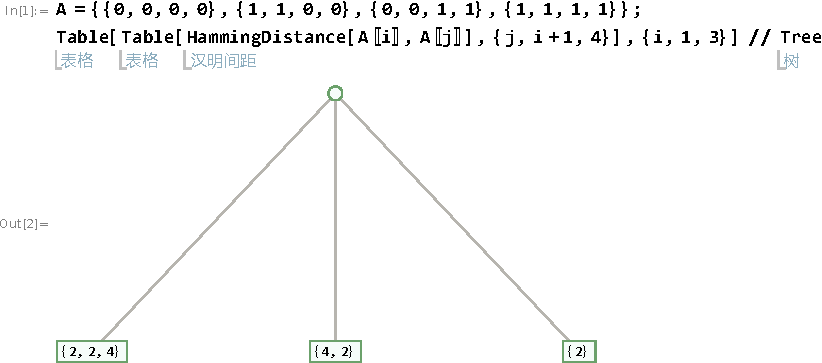
\includegraphics[width=\linewidth]{figure/q31.pdf}
	则$d(C)=\min_{x,y\in C}d(x,y)=2.$
	\end{frame}
	\begin{frame}{问题三}
		\begin{itemize}
			\item 若令$C'=\{0000\textcolor{red}{0},1100\textcolor{red}{1},0011\textcolor{red}{1},1111\textcolor{red}{0}\}$
		\end{itemize}
		由Mathematica:
		\noindent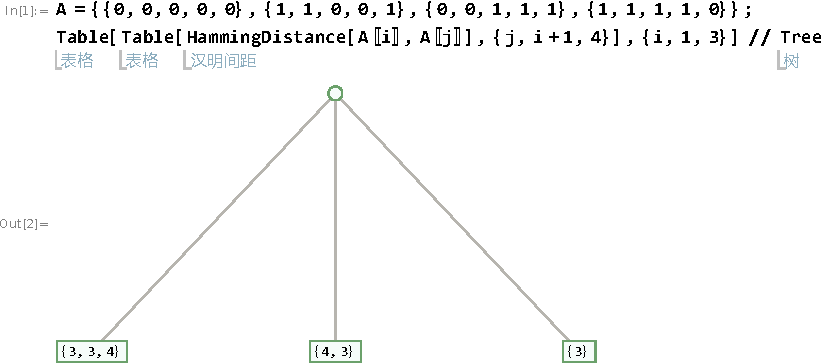
\includegraphics[width=\linewidth]{figure/q3.pdf}
		则$d(C')=\min_{x,y\in C'}d(x,y)=3.$\qed
	\end{frame}
\section{参考文献}
	\begin{frame}
		\frametitle{参考文献}
		\bibliography{ref/ref}
	\end{frame}
	\begin{frame}
		\centering\Huge \color{orange}Thank you!
	\end{frame}
	
\end{document}